\documentclass[conference]{IEEEtran}
\IEEEoverridecommandlockouts
% The preceding line is only needed to identify funding in the first footnote. If that is unneeded, please comment it out.
\usepackage{cite}
\usepackage{amsmath,amssymb,amsfonts}
\usepackage{algorithmic}
\usepackage{graphicx}
\graphicspath{{figures/}}
\usepackage{textcomp}
\usepackage{xcolor}
\usepackage{balance}
\usepackage{url}
\usepackage[hidelinks]{hyperref}
\usepackage[T1]{fontenc}
\def\UrlBreaks{\do\/\do-}
\def\BibTeX{{\rm B\kern-.05em{\sc i\kern-.025em b}\kern-.08em
    T\kern-.1667em\lower.7ex\hbox{E}\kern-.125emX}}
\begin{document}

\title{The Evolution of Lyrics in German Rap}


\author{\IEEEauthorblockN{Luca Schumann}
\IEEEauthorblockA{\textit{lucsc442} \\
\textit{TDDE16}}
}

\maketitle

\begin{abstract}
German rap is a relatively new music genre that has grown quickly in the presence of online streaming. In this work we build a LDA topic model to find five prevalent topics in German rap lyrics. A focus of the work lays on tackling the problems of preprocessing German song texts. We present a timeline that shows how the lyrical landscape in rap has evolved during the last 30 years. It has moved from mainstream music towards battle rap in the early 2000s. In the last decade trap and street rap are taking over the scene. We furthermore show how Sido's change from being a gangsta rapper to being a loving father reflects in his lyrics. Finally, we cluster the artists with help of a 2D visualization of all rappers' lyrical preferences. It shows how almost all rappers of the early years are clustered together, whereas today there appears to be more diversity in the lyrics.
\end{abstract}

\section{Introduction}
This project is about exploring the possibilities of topic modeling German rap lyrics. Probabilistic topic models are (often unsupervised) learning algorithms, designed to find latent structures in large document collections. In this project, we use Latent Dirichlet Allocation (LDA), a generative model, to find the underlying topics in German rap lyrics. It is based on the idea of a generative procedure, in which a text is written with a specific topic or distribution of topics in mind. For each word, a topic from that distribution is then chosen and finally a word from the chosen topic is written. LDA is used to reverse engineer this process and to infer the latent topics responsible for the resulted texts.\\
German rap is a fairly new genre that origined in the 80s and has been through many developments since. \textit{Die Fantastischen Vier} were the firsts to establish rap in German mainstream culture in the early 90s. Driven by influences of American gangsta-rap, the hip-hop record label \textit{Aggro Berlin} (Aggro is slang for being aggressive) was founded in 2001 and introduced a new subgenre, very different from what has been produced so far. Later in the decade, another American import product made its way to Germany. Rappers like \textit{Money Boy} and \textit{Fler} were the firsts to combine trap music with German language. Today, this music style is omnipresent in the Spotify charts.\\
This report presents a LDA model that finds five latent topics in almost 7500 extensively preprocessed songs. The resulting model is used to demonstrate lyrical trends in the past 30 years of German rap music. A 2D visualization is furthermore used to show the {\lq}lyrical distance{\rq} between all analyzed artists. Finally, we inspect the musical career of one particular rapper, namely \textit{Sido}, in more detail. We show how his personal development and career decisions correlate with a change in his lyrical topics over a period of 15 years.\\
The motivation to do this project to see if a) we were able to build an interpretable topic model for German rap lyrics and b) if with the help of this model, we could see the major developments in the hip-hop scene reflected in those lyrics.

\section{Theory}
In this Section, we will introduce some theoretical background that is helpful to better understand the remainder of the report.
\subsection{Latent Dirichlet Allocation} \label{sec:lda}
Latent Dirichlet Allocation (LDA) is a generative probabilistic model that presumes a latent structure in documents consisting of $K$ different topics \cite{hoffman}. Each topic $k$ is characterized by a multinomial distribution $\beta_k$ over the entire vocabulary. The generative process is as follows. For each topic $k$ in $(1,K)$, choose a parameter ${\beta_k \sim\ Dirichlet(\eta)}$ for the topic distribution. A document $d$ is created by first choosing a distribution ${\theta_d \sim\ Dirichlet(\alpha)}$ over the topics. Then, each word $w_{di}$ in the document is generated by first sampling $z_{di}$.\\
1. Draw a topic from the topic distribution of the document:
$${z_{di} \sim\ Multinomial(\theta_d)}$$
2. Generate a word from that topic:
$${w_{di} \sim\ Multinomial(\beta_{z_{di}})}$$
$K$, $\eta$ and $\alpha$ are all adjustable hyperparameters of the model.\\
We can analyze a collection of documents with LDA if we find the posteriors of the various distribution. Since the true posterior is computationally intractable, it has to be approximated with one of many inference methods. Popular methods for this task are variational Bayes \cite{blei} and Gibbs sampling \cite{griffiths}, a Markov Chain Monte Carlo algorithm. The LDA model used in this project utilizes an online variational Bayes algorithm\footnote{https://radimrehurek.com/gensim/models/ldamodel.html}.

\subsection{Principal Component Analysis}
The goal of Principal Component Analysis (PCA), is to find a coordinate system for possibly correlated data points, in which they are linearly uncorrelated \cite{pca_leskovec, pca_jolliffe}. The dimensions with low variance can then be ignored to reduce the dimensionality of the data. To remove the linear correlation between data points, they are transformed such that the covariance between the new dimensions is zero. To do so,\\
1. Center the data $X$ by shifting all points $x_i \in \mathbb{R}^d$ by their mean $\bar{x}$: $${\widetilde{x_i} = x_i - \bar{x}}$$
2. Compute the covariance matrix $\Sigma_{\widetilde{X}} \in \mathbb{R}^{d{\times}d}$\\
3. Eigendecomposition of the covariance matrix: $$\Sigma_{\widetilde{X}} = \Gamma \cdot \Lambda \cdot \Gamma$$
$\Lambda$ is now the (diagonal) covariance matrix in the new coordinate system with eigenvalues $\lambda_i$ as diagonal elements and $\Gamma$ is the transformation matrix. The data can simply be transformed to the new coordinate system by computing $${Y = \widetilde{X} \cdot \Gamma}$$
To reduce the dimensionality of the data to $k$, the transformation matrix $\Gamma$ needs to be truncated before transforming the data. To minimize the information loss, the eigenvectors of $\Gamma$ that correspond to the $k$ largest eigenvalues of $\Lambda$ are kept.

\section{Data}
In this Section, we present the source and selection criteria for the data as well as the preprocessing steps for the songs.

\subsection{Dataset}
First of all, a selection of songs had to be made. To find a balance between relevant artists in the CD era and the streaming era, we decided to combine lists of artists from two sources. We selected all 46 german artists from the Wikipedia list of rappers that sold more than 100,000 albums in Germany \cite{wiki_albums}. The popularity of musicians today, especially rappers, is not only defined by the albums sales, but also the online streams. Therefore we picked all 13 rappers appearing in the Spotify playlist {\lq}Top German Artists of 2020{\rq} \cite{spotify_2020} that were not in the selection yet. To increase the dataset, we chose 18 more subjectively popular rappers, adding up to 77 artists in the end.\\
The lyrics of the artists' songs were then downloaded using the Genius API\footnote{https://docs.genius.com/} with help of Python's \textit{lyricsgenius} package \cite{lyricsgenius}. We excluded feature songs, as it would have been very difficult to seperate which artist sung which part. A lot of the songs are duplicates, since remixes, features and live versions are all included in the genius database. There are furthermore many non-songs in the database, such as commentaries and instrumentals. Luckily, most could easily be ignored by discarding songs that contain brackets, as in \textit{Papa ist da (AsadJohn Remix)}. Few others had to be handled differently, but the final dataset is clean of such occurences. In a first run of the model, songs containing english lyrics formed an individual topic. Upon manual inspection, there were a few songs with parts in english, or even completely in english. Therefore, songs that contain all of the most common english words in the english topic {\lq}the{\rq}, {\lq}you{\rq} and {\lq}and{\rq} were suspected to contain english lyrics and also discarded. The final dataset features close to 7500 songs.

\subsection{Preprocessing} \label{preprocessing}
Preprocessing the song lyrics was an iterative process with many lessons learned. The most basic first step is to remove meta information that is written in brackets from the lyrics, such as \textit{[Hook]}. Next, the songs are tokenized using spacy's German package. Non-alphabetic tokens, stop words and tokens with less than three letters are removed. The rest of the preprocessing is done with Gensim. Bigrams and Trigrams are added and extremes are filtered. Finding the seemingly best values for these tasks was done with the trial and error method.\\
After excluding english songs from the dataset, the model would still find a topic with mostly english stop words. After removing english stop words during preprocessing, the problem was solved. Another problem was many artists' names appearing in the most salient words of some topics. The reason for this, is that some rappers are notorious for talking and singing about themselves in the third person. Rappers with a lot of songs in the dataset would therefore skew the results, although their own name has nothing to do with the message behind their song. To tackle the problem, each artists' name was removed from his or her lyrics. Unfortunately this method is not foolproof, as some refer to themselves by nicknames, e.g. \textit{Ufo361} simply calls himself \textit{Ufo}. As a final tweak of the preprocessing step, a couple of stop words that were not in spacy's German list were manually removed.\\
Tokenizing German text turned out to be a difficult task, with no really satisfying solution. In German texts, all nouns are capitalized, therefore also in spacy's word list. If a word at the beginning of a sentence is capitalized, it is not possible for spacy to tell wether it's a noun or not. Feeding spacy all words in lowercase would also not solve the problem, since it would not recognize the nouns anymore. Additionally, some words have a different meaning depending on wether they are a noun (capitalized) or not. E.g. {\lq}Weg{\rq} means path but {\lq}weg{\rq} means away in German. This appears to be an unsolved problem as of today, as can be read on spacy's Github forum \cite{spacy_issues}. Lemmatization does also not work as well as for english text, but overall the results are good enough to work with them.

\section{Method}
All the code for the project can be found inside the jupyter notebook {\lq}Main{\rq} inside the Github repository\footnote{https://github.com/Lucapaulo/Text-Mining-Project}.\\
First the lyrics of the selected artists are downloaded from the genius API with help of the lyricsgenius package \cite{lyricsgenius} and stored in individual json files. Next, the lyrics are extracted from the json files and some first preprocessing is done: Non-songs, songs with English parts and duplicate songs are dropped, linebreaks and meta information are removed from the lyrics. The remainder is then stored in a data frame together with the release date, artist name and song name.\\
Next, the lyrics are lemmatized using spacy's German word list. Stop words, non-alphabetic tokens and short tokens are additionally removed during this step. Afterwards some manually added stop words, english stop words and rappers' names are removed. The reasoning behind this is explained in Section \ref{preprocessing}. The rest of the preprocessing is done using Gensim. Bigrams and trigrams are added, the tokens are added to the dictionary, tokens that appear to often or too seldom are removed from the dictionary and finally the bag-of-words representation is computed to be stored in the corpus.\\
Now the LDA model is computed given $k=5$ topics and other parameters like a seed, number of passes, eta and alpha. After the model is finished, the topic distribution for each song is computed and added to the data frame. Two more columns are added, one with the majority label of each song and another one with the popularity score from Spotify\footnote{https://developer.spotify.com/documentation/web-api/}, downloaded using the spotipy package \cite{spotipy}. The final data frame is also uploaded to the repository as \textit{all\_songs.pkl}, so to reproduce the results the data does not need to be redownloaded. The plots shown in this report are all created from that data frame, the code for them is also in the notebook.

\section{Results} \label{results}
The results are split into four parts, the first being about the discovered topics and the others about further analysis of the dataset.

\subsection{Model and Topics}
The most popular models for topic modeling are Non-negative matrix factorization (NMF) and the previously introduced LDA, see Section \ref{sec:lda}. The first task was to find the best model and number of topics for the project. To achieve this, the coherence scores for a NMF and a LDA model with 3-15 topics were computed. The LDA models scored consistently better than the NMF models. In a manual comparison of a NMF model to a LDA model, the LDA model also gave more interpretable results. We therefore continued working with LDA models. A selected subset of the test results can be found in the jupyter notebook {\lq}Experiments{\rq}.\\
Previous work has shown \cite{evaluation} that manual quality assessment is better suited for topic modelling song lyrics, which is why we manually chose the best number of topics. As a result, five topics is the best choice from our point of view, since the resulting topic clustering delivers the greatest expressiveness compared to the other options. Later in this Section, we will compare a {\lq}good{\rq} to a {\lq}bad{\rq} model to illustrate this point.\\
Eta and alpha were fine tuned using the coherence value as measure, which lead to terrible results. We manually selected {\lq}auto{\rq} as the best value for both parameters, which means that the model learns these parameters automatically. Our results confirm Newman et al.'s observation \cite{evaluation} that coherence measures are not optimal to assess the quality and interpretability of topics in music lyrics.\\
The final iteration of the model found five topics that we named {\lq}Street{\rq}, {\lq}Sex \& Party{\rq}, {\lq}Love \& Life{\rq}, {\lq}Competition{\rq} and {\lq}Lifestyle{\rq}. To show the limit of the classification, we manually labeled one song of every artist with the expected topic. The model managed to find the expected label in 57 of 77 songs (74\%). Table \ref{tab:topics} shows the eleven most salient terms for each topic, translated to English. It strucks right away that many English terms are used in the lyrics, especially in the {\lq}Lifestyle{\rq} topic, were seven words are not translated. Interestingly, there are none in {\lq}Street{\rq} or {\lq}Love \& Life{\rq}. Some words such as \textit{see}, \textit{man} or \textit{yeah} make it in the top terms of multiple categories. \textit{Come} for example even appears twice very high up in the {\lq}Sex \& Party{\rq} list. In the original German list the verb is once capitalized, which is the reason for it appearing twice. As mentioned in Section \ref{preprocessing}, spacy does not recognize capitalized non-nouns at the beginning of sentences correctly.

\begin{table}[htbp]
\caption{11 Most Salient Terms for each Topic, Translated}
\begin{center}
\begin{tabular}{|c|c|c|c|c|}
\hline
\textbf{Street}&\textbf{Sex \& Party}&\textbf{Love \& Life}&\textbf{Competition}&\textbf{Lifestyle} \\
\cline{1-5}
\hline
brother & baby$^{\mathrm{O}}$ & life & rapper$^{\mathrm{O}}$ & bro \\
\hline
money & come & (to) love & rap$^{\mathrm{O}}$ & bitch$^{\mathrm{O}}$ \\
\hline
street & know & world & see & money$^{\mathrm{O}}$ \\
\hline
mom & come & see & come & money \\
\hline
head & yeah$^{\mathrm{O}}$ & know & boy & bitches$^{\mathrm{O}}$ \\
\hline
boys & say & stay & yeah$^{\mathrm{O}}$ & yeah$^{\mathrm{O}}$ \\
\hline
out & please & stand & bitch$^{\mathrm{O}}$ & cash$^{\mathrm{O}}$ \\
\hline
life & party$^{\mathrm{O}}$ & man & fuck & gang$^{\mathrm{O}}$ \\
\hline
block & drag$^{\mathrm{M}}$ & think & man & bro \\
\hline
away & night & just$^{\mathrm{M}}$ & king$^{\mathrm{O}}$ & fuck \\
\hline
run & club$^{\mathrm{O}}$ & heart & people & Gucci$^{\mathrm{O}}$ \\
\hline
\hline
\multicolumn{5}{l}{$^{\mathrm{O}}$Original, not translated $^{\mathrm{M}}$Multiple translations possible}
\end{tabular}
\label{tab:topics}
\end{center}
\end{table}

\begin{figure}[!t]
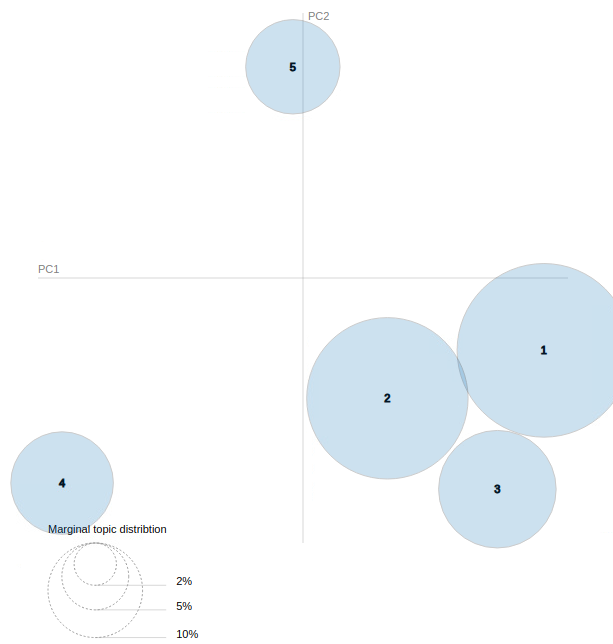
\includegraphics[width=\linewidth]{figures/topic_dist.png}
\vspace*{-8mm}
\caption{The intertopic distance map for all five topics. The distance is computed as the Jensen-Shannon divergence and projected to 2D space. 1: Love \& Life, 2: Competition, 3: Street, 4: Lifestyle, 5: Sex \& Party.}
\label{fig:topic_dist}
\end{figure}

\begin{figure}[!t]
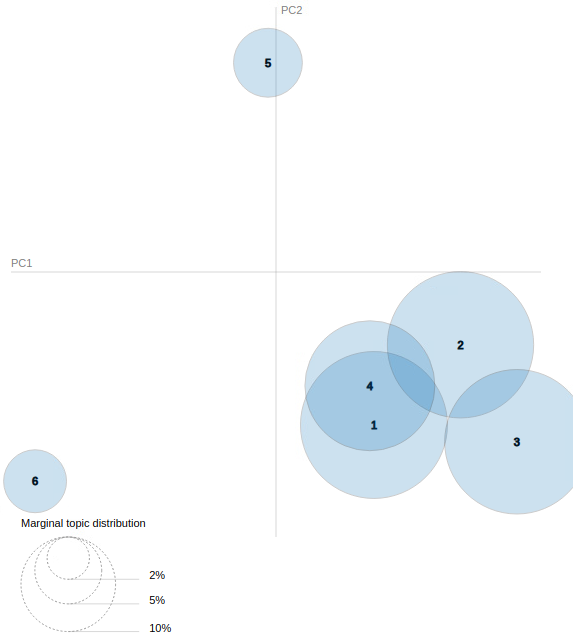
\includegraphics[width=\linewidth]{figures/topic_dist_bad.png}
\vspace*{-8mm}
\caption{The intertopic distance map for a discarded model with six topics. The distance is computed as the Jensen-Shannon divergence and projected to 2D space.}
\label{fig:topic_dist_bad}
\end{figure}

Figure \ref{fig:topic_dist} shows the intertopic distance map, visualized by the Python implementation of the LDAvis tool \cite{sievert-shirley-2014-ldavis}. The five topics are drawn as circles in 2D space, by first computing the intertopic distances and then multiplying those with the transformation matrix obtained from PCA. Each topic's overall frequency is depicted by the size of the respective blob. The topics {\lq}Lifestyle{\rq} and {\lq}Sex \& Party{\rq} stand out as the smallest, with 11.8\% and 10\%, respectively. They also have a huge gap between them and the other topics. The other three topics are rather close in comparison, but still with a noticeable distance between each other. The next largest topic is {\lq}Street{\rq} with 15.4\%, followed by {\lq}Competition{\rq} with 29.1\% and finally {\lq}Love \& Life{\rq}, which is assigned to 33.7\% of all tokens.\\
In Figure \ref{fig:topic_dist_bad} you can see the intertopic distance map for a model trained to use six topics. This serves as a comparison to the distance map of the final model. The two smallest blobs are assigned 4.4\% and 5.3\% of all tokens, respectively. The topics 1, 2 and 3 are arranged similarly as in Figure \ref{fig:topic_dist}, albeit with a shorter distance inbetween. Additionally, there is topic 4, which is very close to topics 1 and 2, indicating a major overlap with both topics.

\subsection{Topics in Rap over Time}
In this section we visualize the development of German hip-hop lyrics over the last 30 years. Figure \ref{fig:timeline} depicts the average topic distribution of all songs that were released in the respective year. Since the number of songs released differs each year, the data is normalized to better capture the bigger picture. Note that they years until 2003 contain less than 100 songs each, whereas each year after 2011 has more than 400 songs in the dataset. This imbalance is not due to a poorly selected subset of artists, but rather due to the rapid growth in popularity of German rap in the last 10 years \cite{musikindustrie}. Multiple trends can be seen in this graphic. First of all, an increase of the topic {\lq}Competition{\rq} with a peak in 2005, followed by a steady decline until 2018. Next, we observe a fast growth of the {\lq}Lifestyle{\rq} topic since 2010, as well as a moderate growth of {\lq}Street{\rq} rap between 2008 and 2018. Throughout most years, {\lq}Love \& Life{\rq} appears to be the most dominant topic.\\
This method automatically gives higher influence to artists with more songs in a release year. It also disregards the music preferences of the audience. Figure \ref{fig:w_timeline} is meant to capture the preferred topics by the consumers, by weighting each song with its Spotify popularity score. The score is downloaded for each song from the Spotify API using the \textit{spotipy} package \cite{spotipy}. It measures the current popularity of a song on a scale from 0 to 100. To increase the influence of more popular songs on the graphic, we extended the scale to 1000. An exponential function maps e.g. the score 100 to 1000 or 90 to ca. 500. Note that the vast majority of scores are in the middle of the scale, so the weighting is not as strong as it may seem on the first look. Compared to the unweighted graphic, we immediately notice a much higher share of the topics {\lq}Street{\rq} and {\lq}Sex \& Party{\rq} throughout the entire timeline. The topics {\lq}Love \& Life{\rq} and {\lq}Competition{\rq} on the other hand seem to be less popular. {\lq}Lifestyle{\rq} is mostly unchanged by the weighting.

\begin{figure}[!t]
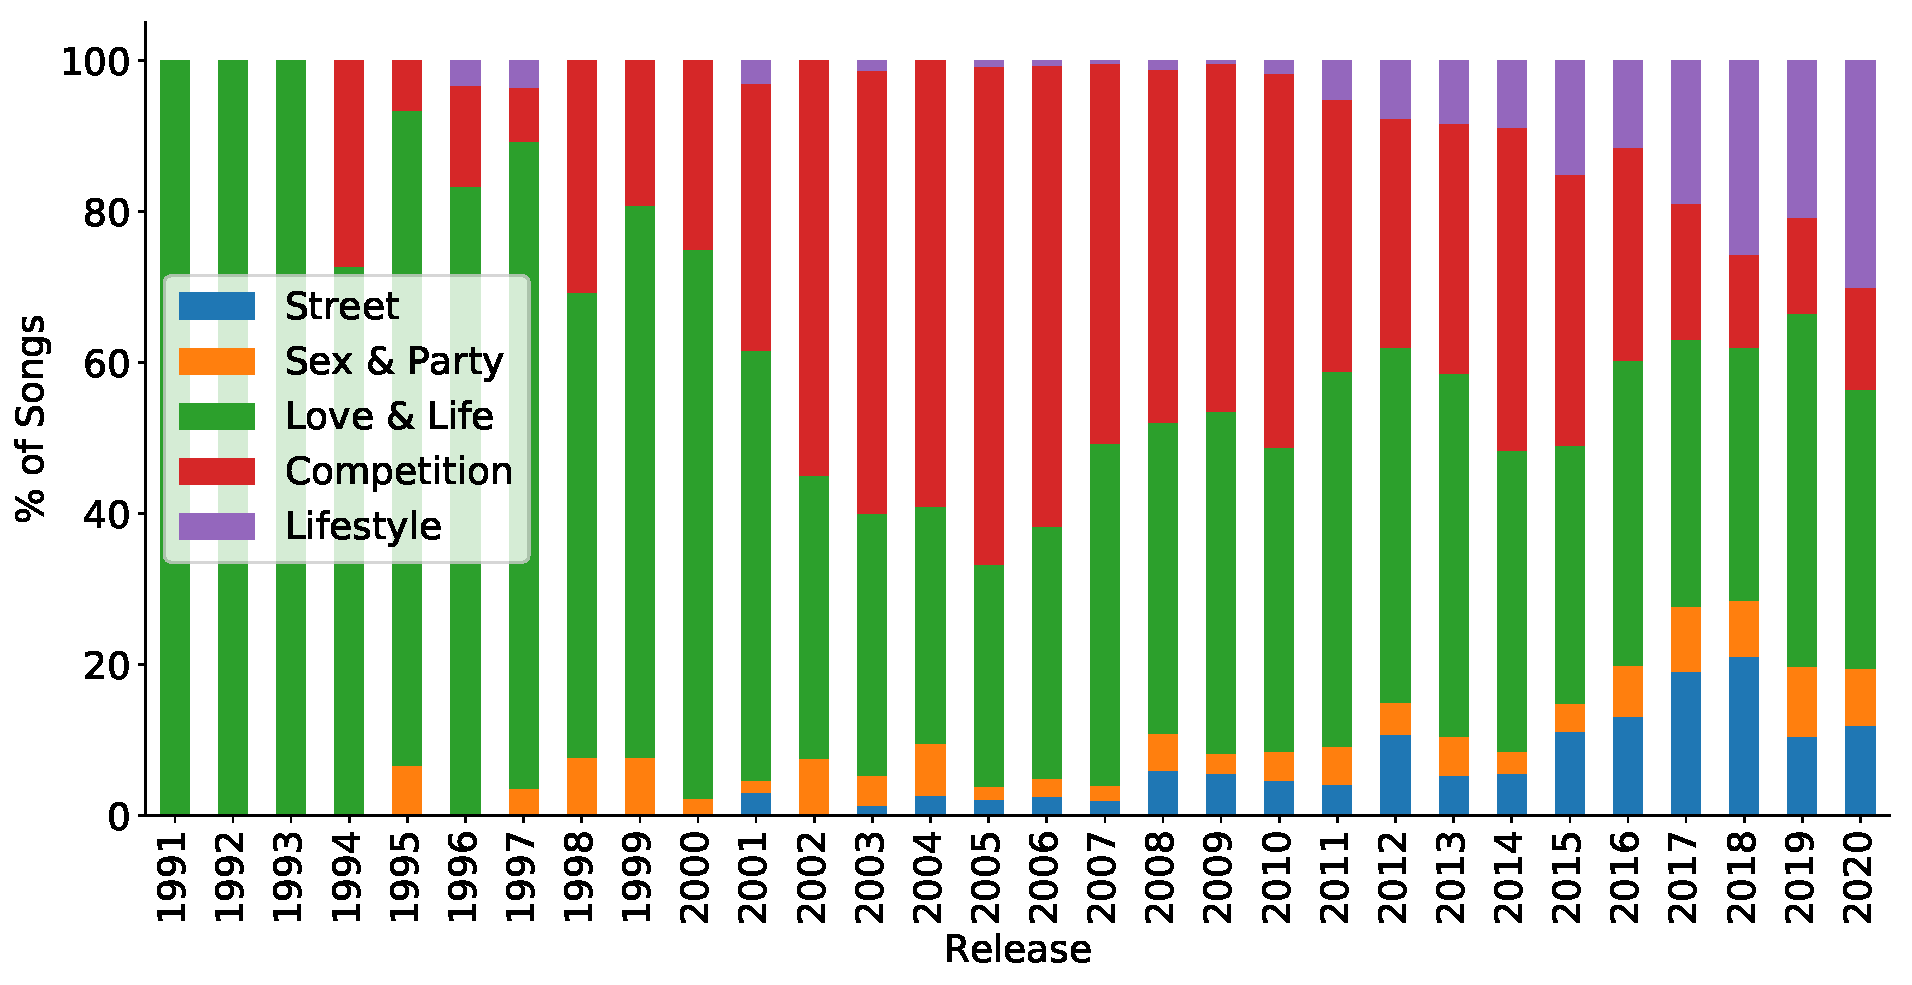
\includegraphics[width=\linewidth]{figures/timeline.pdf}
\vspace*{-8mm}
\caption{Normalized timeline of the average topic distribution in the lyrics of songs released between 1991 and 2020.}
\label{fig:timeline}
\end{figure}

\begin{figure}[!t]
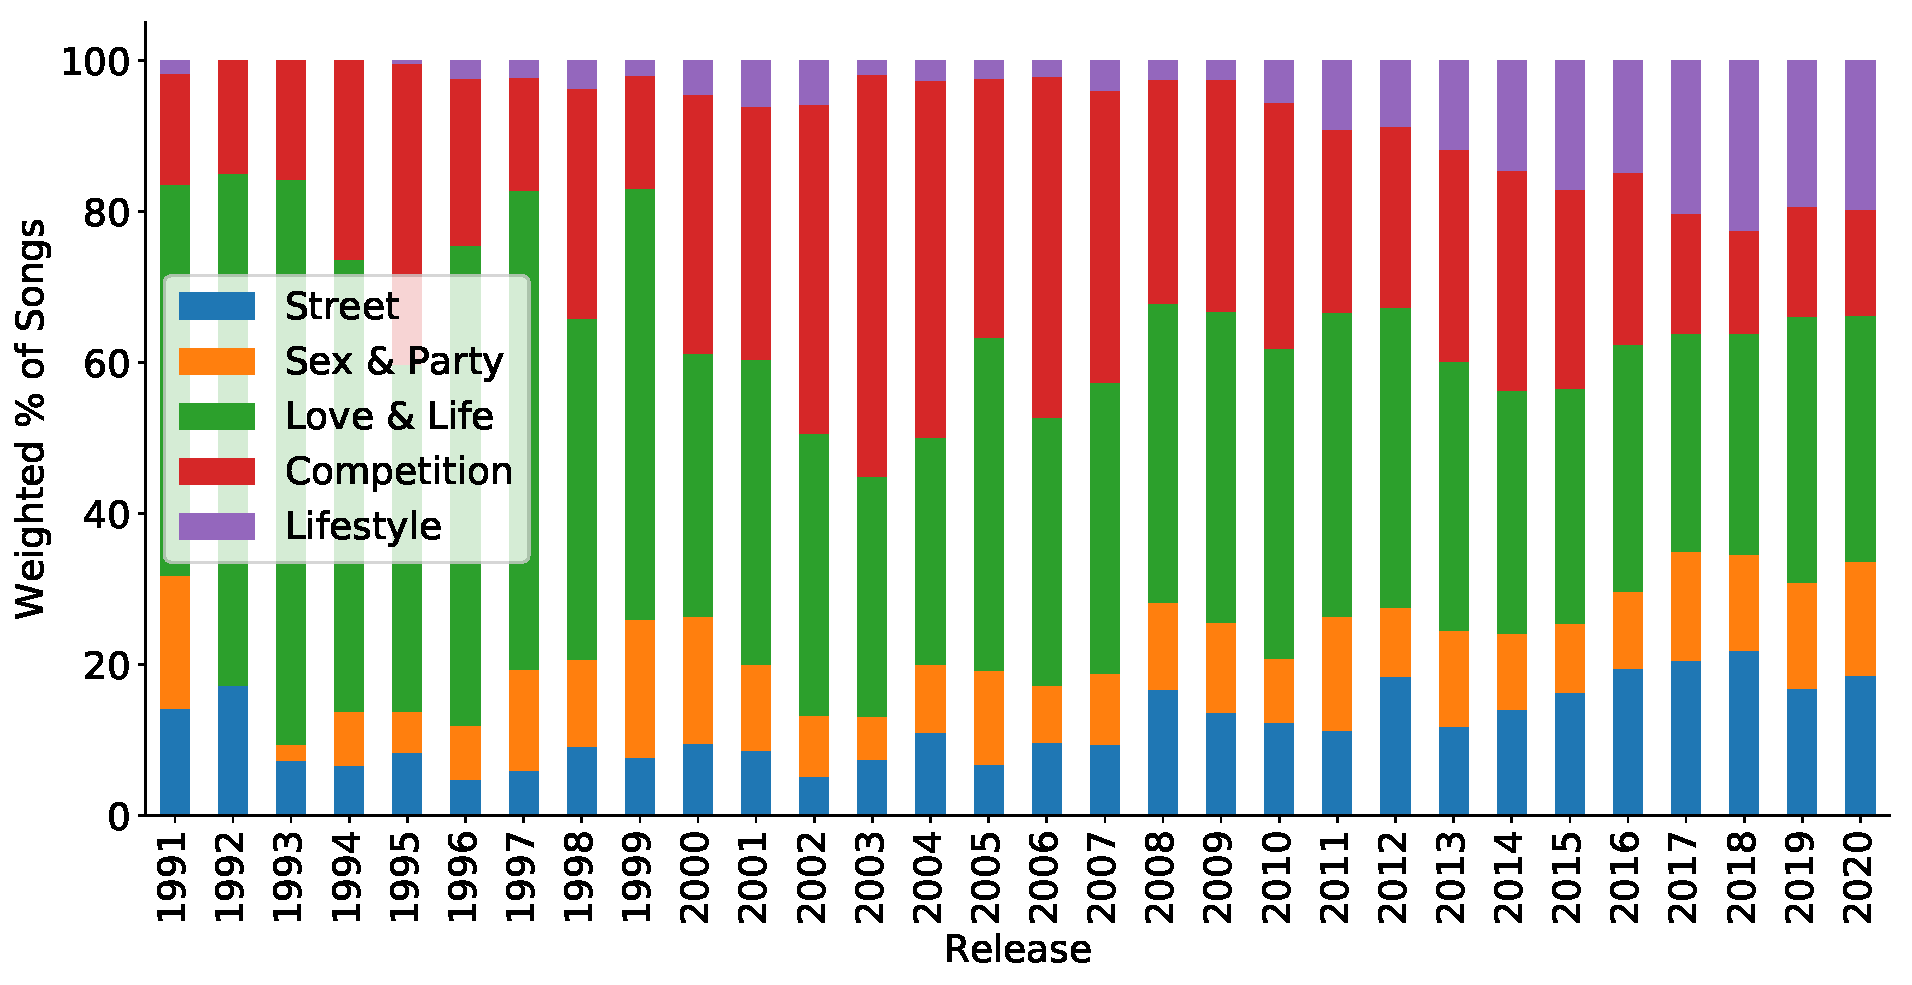
\includegraphics[width=\linewidth]{figures/w_timeline.pdf}
\vspace*{-8mm}
\caption{Normalized timeline of the average topic distribution in the lyrics of songs released between 1991 and 2020. Songs are weighted by their popularity score on Spotify.}
\label{fig:w_timeline}
\end{figure}

\subsection{Sido's Story - Underground to Mainstream}
In this part we want to lay the focus on one particular rapper, namely \textit{Sido}. We chose \textit{Sido} for this, because he is known as a prime example of someone that turned their life around. We elaborate more on this later in the discussion. Although he started his music career in the late 90s, his solo career did not start before the end of 2003, which is why the graph in Figure \ref{fig:sido} starts in 2004. 2004 to 2007 we can see an upwards trend of the topics {\lq}Competition{\rq} and {\lq}Sex \& Party{\rq}, contributing to almost 80\% of the rapper's lyrics in 2007. The following years, there is a decline of the two topics, which are being contested by {\lq}Love \& Life{\rq}. 2019 {\lq}Love \& Life{\rq} makes up around 60\% of the lyrics on its own. {\lq}Street{\rq} appears to always play a role in his songs, hovering around 15\% throughout the years. {\lq}Lifestyle{\rq} has the lowest contribution to his music in each year, apart from a 20\% peak in 2012.

\begin{figure}[!t]
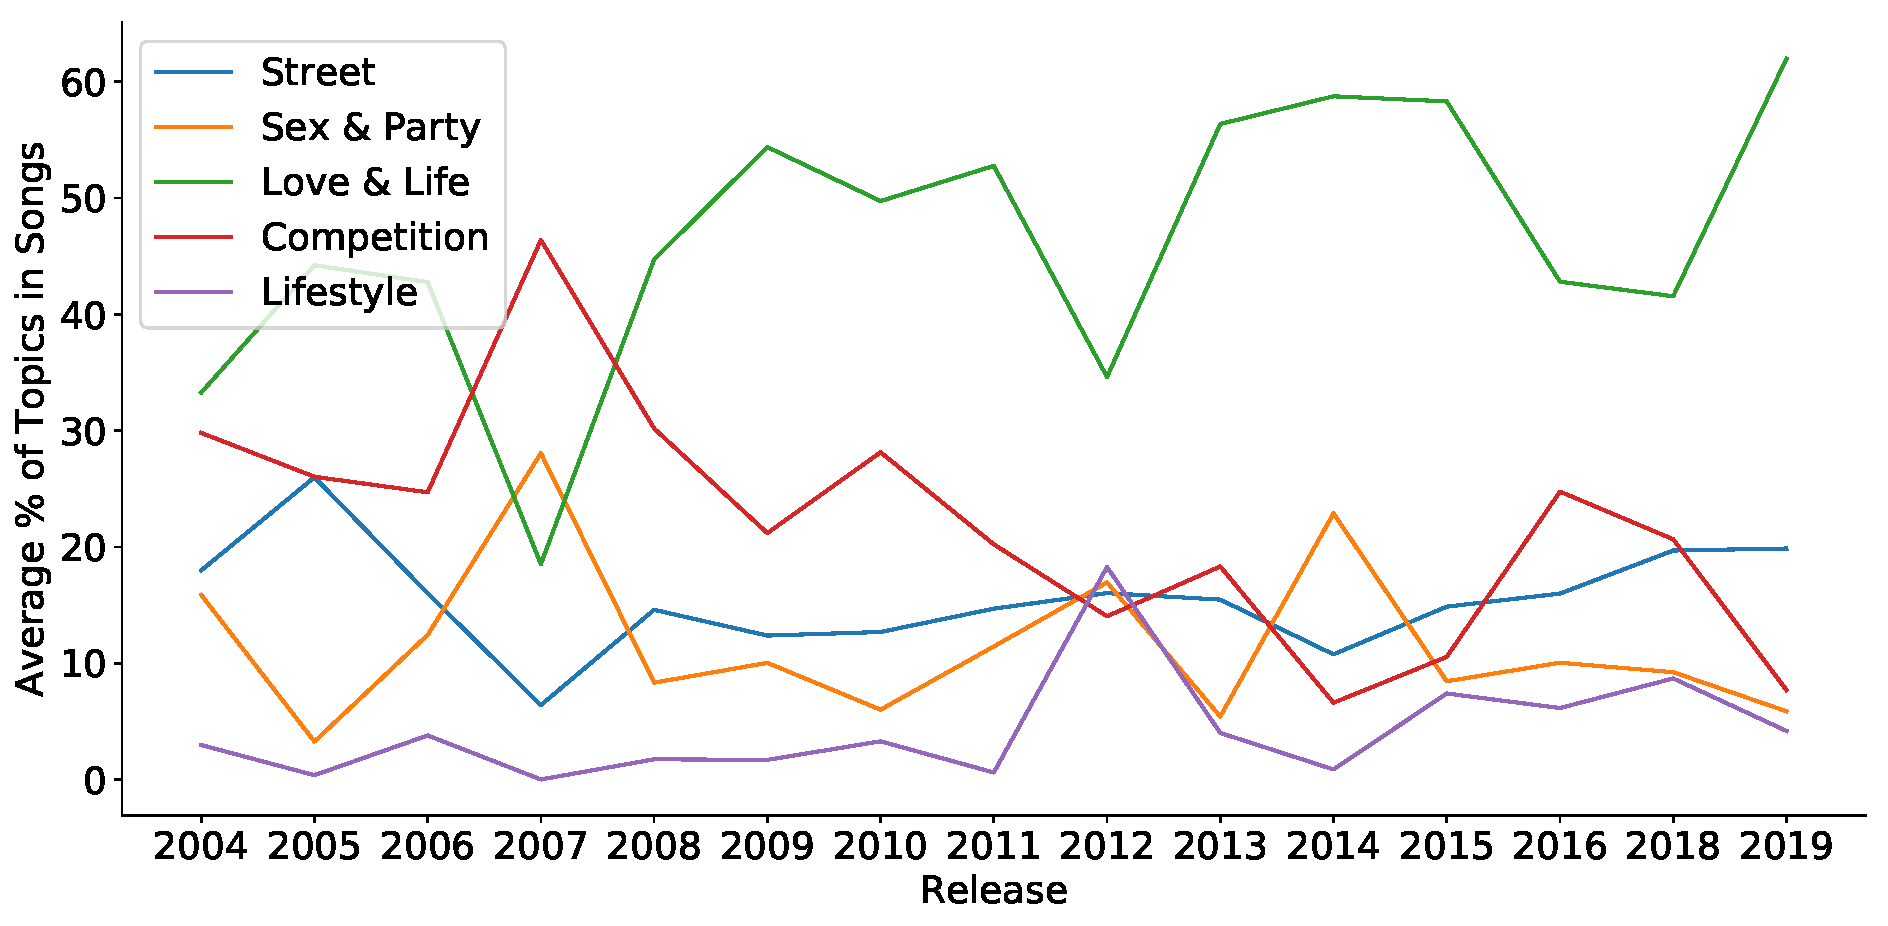
\includegraphics[width=\linewidth]{figures/sido.pdf}
\vspace*{-8mm}
\caption{The average percentage of topics in \textit{Sido}'s songs between 2004 and 2019.}
\label{fig:sido}
\end{figure}

\subsection{An Artist Overview}
The last part of this section focusses on the similarity of the lyrics of all analyzed artists. Figure \ref{fig:scatter} visualizes the distance between the artists in 2D space. The average distribution of the artists' songs for each of the five topics were the original vectors in 5D space, reduced to two dimensions using PCA. The dots are colored with the majority label of each artist's lyrics. We can see a large {\lq}Love \& Life{\rq} cluster on the left side of the graph, that makes up more than half of the entire space. The upper part is dominated by the {\lq}Competition{\rq} topic, and the right side is shared by {\lq}Street{\rq} and {\lq}Lifestyle{\rq}. {\lq}Sex \& Party{\rq} as the majority label does not show up in an individual cluster, it only features two artists that are rather separated.

\begin{figure}[!t]
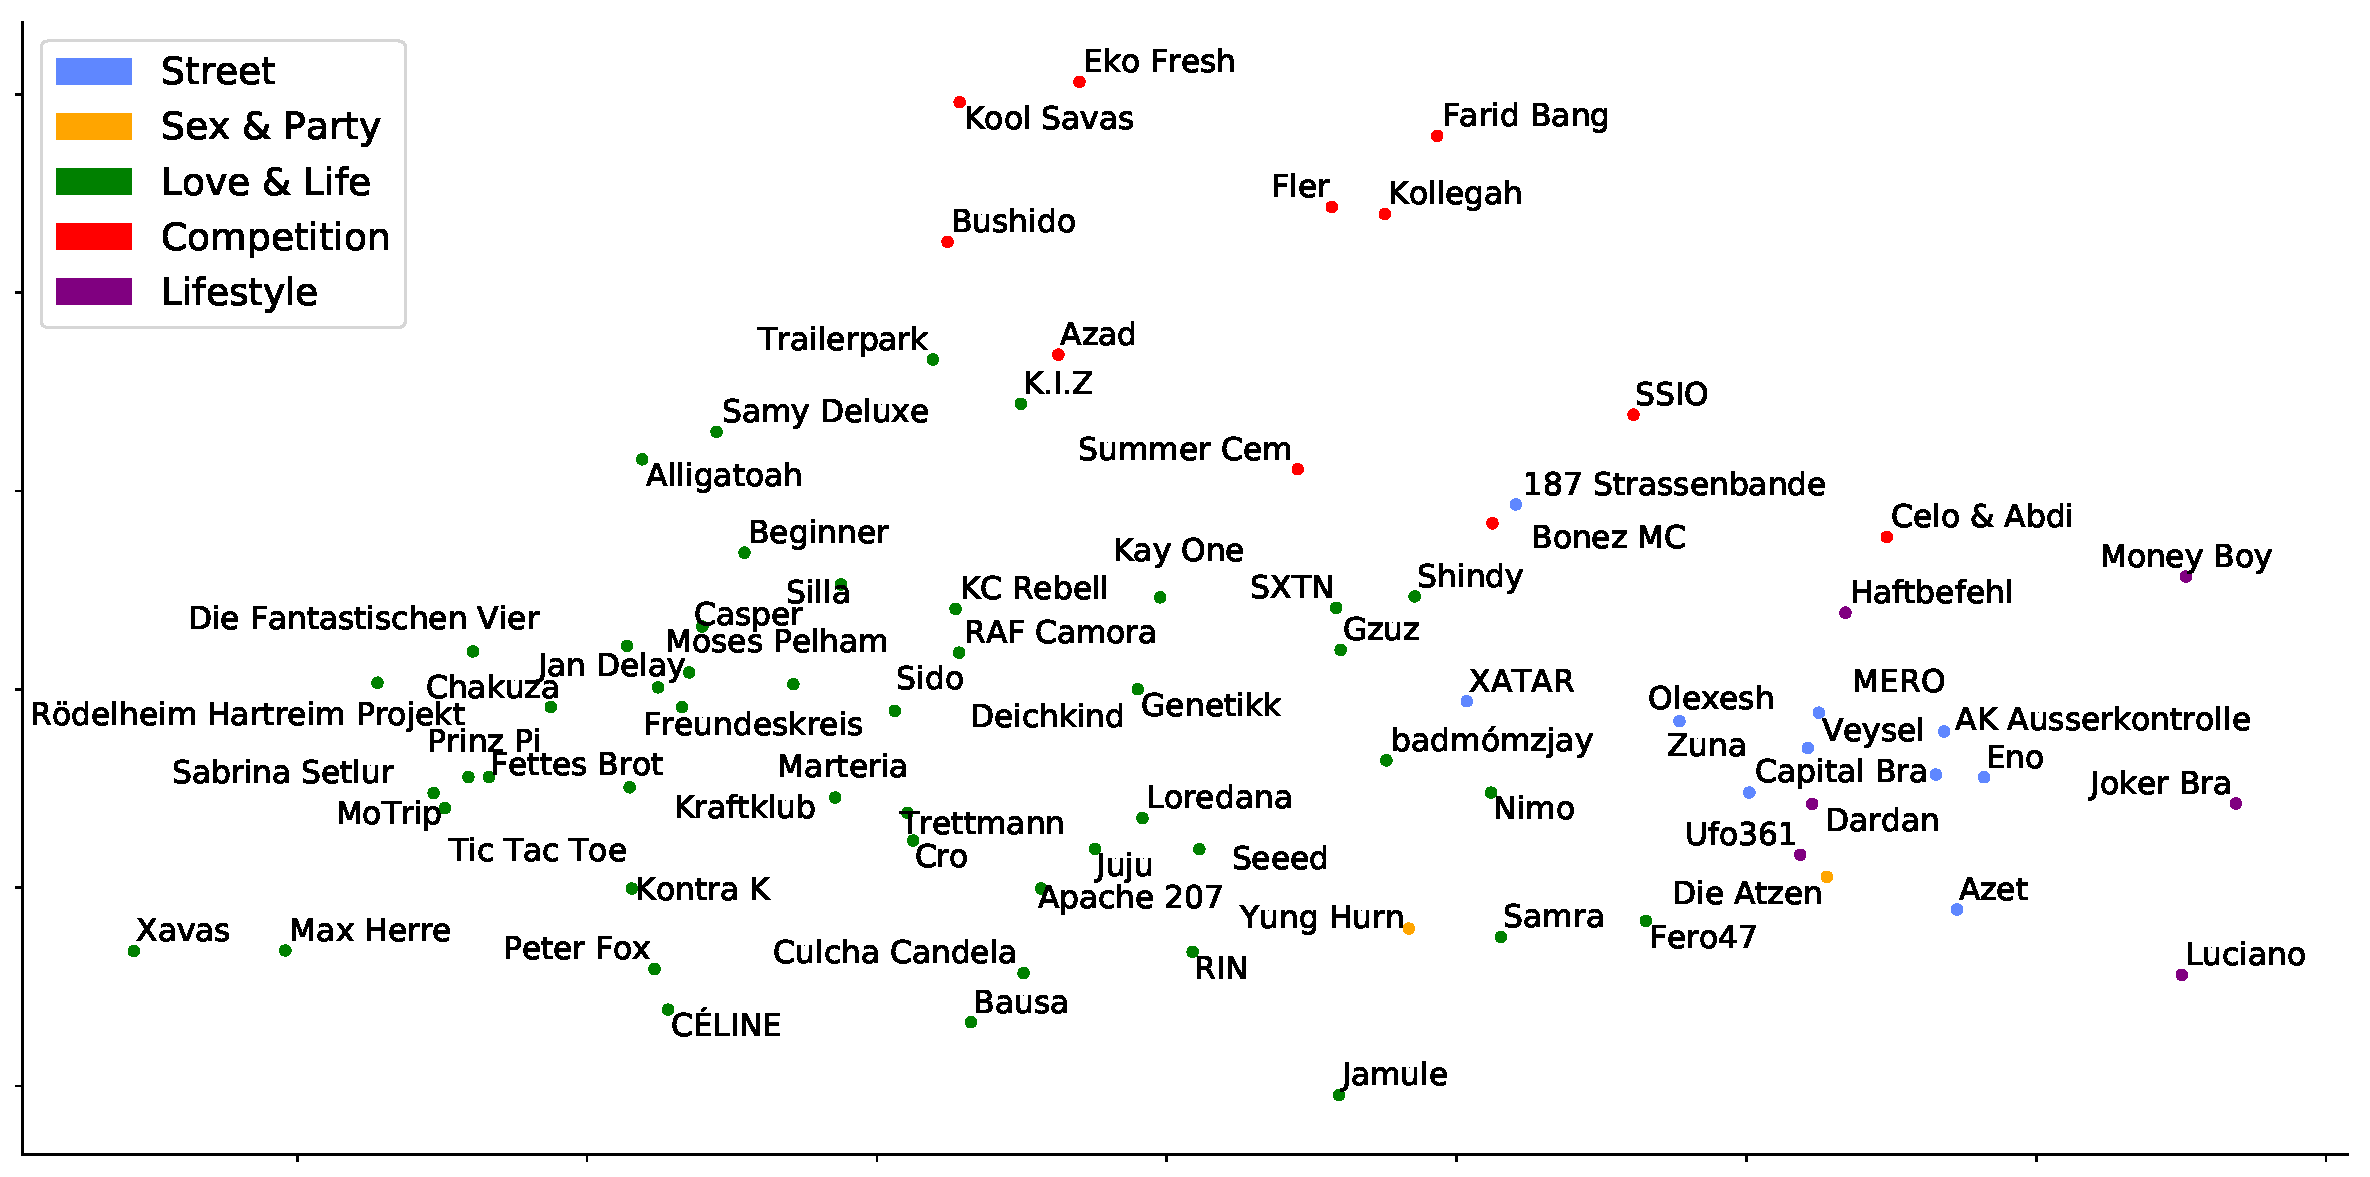
\includegraphics[width=\linewidth]{figures/scatter.pdf}
\vspace*{-8mm}
\caption{A 2D visualization of the average topic distribution in each artist's lyrics. The dots are colored by the majority label.}
\label{fig:scatter}
\end{figure}

\section{Discussion}
\subsection{Analysis}
In this subsection we will give an interpretation to the previously shown results of section \ref{results}.

\subsubsection{The Topics} \label{discussion_topics}
The choice for the correct number of topics is of most critical importance for a good topic model. We eventually sticked to five topics, as it gave the best balance between expressiveness and quality of results. Intuitively, a larger topic number improves the ability of the model to correctly assign a topic to a song. On the other hand, clogging the graphs with 20 different topics makes them harder to interpret, so instead we decided to keep the topic number small and the topics broader. The sizes of each topic vary to a reasonable extent, so that no topic is underrepresented. The intertopic distances are also large enough, such that there is not too much overlap between them, but a relatively clear distinction. Other models have shown far worse results, with extremely niche/broad topics or heavily overlapping topics, as shown on the basis of the six topic example in Figure \ref{fig:topic_dist_bad}.\\
Table \ref{tab:topics} is meant to help understand the content of the topics better. Some of these words seem not to fit the topic on the first read, because they may have a specific meaning in rap culture. E.g. when \textit{king} is mentioned in rap lyrics, the meaning is supposedly more often \textit{king of rap} or \textit{king of the streets}, than that an actual monarch is meant. The difference in the number of English and slang words between the topics can potentially mean that language has an influence on the topic choice. Two sentences with the same meaning but a different word choice could be assigned to different topics. In the best case, this problem is handled by the model using the bag-of-words representation of tokens. Furthermore, the word \textit{yeah} could have been added to the stop word list, but it is hard to decide wether it really belongs there.

\subsubsection{Rap over Time} \label{discussion_timeline}
The first rappers to lift the genre to mainstream media, had to sing about topics that the people knew from other popular music at the time, to make them familiar with it. It is therefore no surprise, that {\lq}Love \& Life{\rq} is so dominant at the beginning in the 90s. Artists like \textit{Die Fantastischen Vier}, \textit{Tic Tac Toe} and \textit{R\"odelheim Hartreim Projekt} peaked at that time.
The rise of the {\lq}Competition{\rq} topic in both Figures \ref{fig:timeline} and \ref{fig:w_timeline} strongly correlates with an interesting development in the German rap scene: The first rivalries (\textit{beefs}) that were carried out in public via battle-rap songs. The first big beef was between \textit{Azad} and \textit{Samy Deluxe} in 2001. \textit{Azad} provoked \textit{Samy Deluxe} in his song {\lq}Gegen den Strom{\rq} (against the stream), who then reacted with his disstrack {\lq}Rache ist s\"u\ss{\rq} (revenge is sweet), which then again was countered by \textit{Azad} with {\lq}Samy De Bitch{\rq}. This is just one of countless battles that took place \cite{battles}, with a peak after 2004, where famous rapper \textit{Bushido} left his record label \textit{Aggro Berlin} with help of the criminal Abou-Chaker clan \cite{abou-chaker}. Brawls and shootings between rappers from Frankfurt and Berlin were also not uncommon at that time \cite{schlaegerei}.\\
{\lq}Lifestyle{\rq} is a topic mainly represented by artists of the trap genre, which started to establish in Germany with artists like \textit{Money Boy}, \textit{RIN}, \textit{Yung Hurn} and \textit{Ufo361}. The growing popularity of this subgenre is also underlined by the fact, that each of the just named artists can be found in Spotify's {\lq}Top Artists of 2020{\rq} playlist \cite{spotify_2020}.\\
Street as a lyrical topic has existed for a long time in Germany, as can be seen in \ref{fig:w_timeline}, but has been through a revival that started with Haftbefehl in 2009. This revival phase of street rap was amplified by many now prominent street rappers like \textit{Bonez MC}, \textit{Gzuz} and \textit{RAF Camora}\cite{strassenrap}. Figure \ref{fig:timeline} also shows, that the volume of songs representing this style has only increased since then. From the popularity chart we can take away that the listening preferences of Spotify consumers show a strong bias towards the topics {\lq}Street{\rq} and {\lq}Sex \& Party{\rq}. Not only recent songs, but also older ones featuring those topics seem to be more popular nowadays compared to contemporaneously produced songs.

\subsubsection{Sido}
The radical change in the lyrics depicted in Figure \ref{fig:sido} correlates with \textit{Sido}'s development as an artist. Until the start of his solo career, he was wearing a chromium skull mask and known as a gangsta rapper that would sing about drugs, sex and violence. His first album as a solo artist was furthermore heavily criticised and indexed \cite{urteil} by the \textit{Federal Review Board for Media Harmful to Minors} \cite{bpjm} because of misogynous and drug-glorifying texts. Since then, he has taken off the mask, fought his heroin addiction and started to move towards an overall more tame personality. In 2013, he also became father, which became an important motive in some of his later songs after. Today, the rapper is regularly represented in the charts with rather {\lq}soft{\rq} songs, often featuring Pop artists \cite{sido_charts}. 2019 he even appeared as a coach in the popular TV show \textit{The Voice of Germany}.

\subsubsection{Overview}
The largest part of rappers in Figure \ref{fig:scatter} being labeled as mainly {\lq}Love \& Life{\rq} is no surprise. First of all, it is the most prevalent topic in the model. Secondly, the topic contains many common words, such as (translated) to know, to see or to say. It is noticeable, that almost all of the artists that were active in the 90s in the set are inside the green cluster, most even very far on the left. Some examples for that are \textit{Fettes Brot}, \textit{Tic Tac Toe}, \textit{R\"odelheim Hartreim Projekt} and \textit{Die Fantastischen Vier}.\\
The top side of the graph features rappers like \textit{Fler}, \textit{Bushido} and \textit{Kollegah} that are often involved in rap battles \cite{battles}. Most of them also have a career going for 15 years or longer, which means they were active during the {\lq}Competition{\rq} peak seen in Section \ref{discussion_timeline}. This red cluster is a strong indication that the {\lq}Competition{\rq} topic is correctly extracted from the texts.\\
The only representatives of {\lq}Sex \& Party{\rq} as the majority label here are \textit{Yung Hurn} and \textit{Die Atzen}. Both sing almost exclusively about drugs in \textit{Yung Hurn's} case or about party in \textit{Die Atzen's} case, which also makes their labels reasonable.\\
The artists \textit{Gzuz} and \textit{Bonez MC} are very close to each other as well as to their group project \textit{187 Strassenbande}, despite all three having a different majority label. This can be interpreted as an even distribution of three topics in the three artists' songs.\\
Finally, the right side of the graph features many active street rappers \cite{strassenrap} such as \textit{Capital Bra}, \textit{Mero} and \textit{Ufo361}. Purple colored dots are also spread around in the same area, which points towards a strong correlation of the topics {\lq}Street{\rq} and {\lq}Lifestyle{\rq}.

\subsection{Limitations \& Future Work}
With more time and work the preprocessing could be further improved by tackling the already mentioned problems. These include smaller influences on the results like removing rappers' nicknames but also bigger ones like improving the quality of stemming. The different language styles of rappers are also a limitation, but since the LDA model uses the bag-of-words representation of the tokens, it should be able to understand the context of those words to an extent. The dataset could also be bigger than it is right now. One option would be to include feature songs and seperate the parts of each artist for the analysis of the individual topic preferences. Another one would be to simply increase the number of rappers in the dataset. Time is mostly the limiting factor here, since downloading lyrics from the genius API is very slow and aborts regularly, resulting in many restarts.\\
The small number of topics is another limiting factor, as they do obviously not cover everything and are too broad in some cases. As explained in Section \ref{discussion_topics}, this choice was made to have more expressive results to present. For a more in depth analysis of lyrics the number of topics could be increased in future work.\\
The LDA model can not only be used to find topics in the dataset that built the model, but also in unseen songs. In the jupyter notebook there is already an implementation of a method that can do this. This makes the possibilities to further expand this project manifold. It could for example be expanded to a platform that suggests lyrically related artists or songs to ones' preferences. The project could also be extended to validate the model using unseen, labeled data.

\subsection{Related Work}
There has already been a lot of previous work in the topic of analyzing song lyrics. In a similar work, Sasaki et al. \cite{sasaki} used LDA to extract the weights of five latent topics for each song in their data. The authors used Japanese songs for their model, our work extends theirs to German lyrics.\\
Another alike approach from Tsukuda et al. \cite{tsukuda} proposes a novel method to model song lyrics which incorporates the artists' tastes for topics.\\
Kleedorfer et al. \cite{kleedorfer} use NMF to identify topic clusters in mostly English lyrics. We find out that NMF performs worse for our application, which is why we use LDA instead.\\
Sterckx et al. \cite{sterckx} use the kurtois metric to assess the quality of a topic model for lyrics, as it strongly correlates with manual topic quality scores. To incorporate their results, we complement the coherence score measure with a manual assessment of the optimal parameters.\\
Work on German song lyrics is very limited. Roman Schneider \cite{schneider} created a corpus of German lyrics together with linguistic features and extralinguistic metadata. His work is different in content and exclusively focuses on pop songs, wheares this project analyzes songs of the rap genre.

\section{Conclusion}
We came to the conclusion that preprocessing song lyrics is an elaborate task which requires careful manual inspection. In addition, lemmatization for German texts seems to still have some problems, making the task even harder.\\
Our work proves that topic modeling for German rap lyrics is indeed possible and yields promising results. LDA seems well suited for this task, as it performs better than NMF in our experiments.\\
We have shown how battle rap, trap music and street rap shaped the lyrical landscape of German hip-hop over 30 years. We could furthermore see, how \textit{Sido}'s transition from a violent gangsta rapper to a mainstream artist reflects in his song texts. Finally, we have presented an overview of the most popular rap artists of German language and their lyrical preferences.

{
\balance{
  \bibliographystyle{IEEEtran}
  \bibliography{report.bib}
  }
}
\end{document}
